\section{Analisis en CA}

\subsection{BJT}
Un amplificador en emisor común (EC), tiene al emisor como terminal común, o
tierra, ante una señal de ca. Los amplificadores en EC tiene una alta ganancia de
voltaje y una alta ganancia de corriente \cite{Floyd}.

\begin{figure}[!ht]
\centering
\includegraphics[scale=0.30]{diagramas/figura17.eps}
\caption{Amplificador en emisor común.}
\label{figura17}
\end{figure}

La \textbf{figura~\ref{figura17}} muestra un amplificador en emisor común con
polarización utilizando un divisor de voltaje y capacitores de acoplamiento
$C_1$ y $C_3$ en la entrada y salida, y un capacitor de puenteo, $C_2$, del
emisor a tierra. La señal de entrada, $V_{\text{ent}}$ está acoplada
capacitivamente a la base; la señal de salida, $V_{\text{sal}}$, está acoplada
capacitivamente del colector a la carga. La salida amplificada está desfasada
$180^{\circ}$ con respecto a la entrada. Como la señal de ca se aplica a la base
como entrada y se toma en el colector como salida, el emisor es común tanto para
las señales de entrada como de salida. No hay señal en el emisor porque el
capacitor de puenteo pone efectivamente al emisor en cortocircuito con tierra a
la frecuencia de la señal. Todos los amplificadores combinan tanto la operación
en ca como en cd.

\subsubsection{Calculo de los parámetros del amplificador}
Para hallar los valores del amplificador en emisor común con divisor de voltaje
calculados en la anterior sección se calculan los siguientes valores:

\begin{enumerate}
\item Resistencia interna del generador de funciones:
\begin{equation*}
    R_s = 350[\Omega]
\end{equation*}
\item Resistencia de ca en el emisor:
\begin{equation*}
    r_e^{'} \cong \frac{25[m{\text{V}}]}{I_E}
            = \frac{\num{25e-3}[\text{V}]}{\num{36.72e-3}[\text{A}]}
            = 0.6808[\Omega]
\end{equation*}
\item Resistencia de entrada en la base:
\begin{equation*}
    R_{\text{ent(base)}} = \beta_{\text{ca}}\,r_e^{'}
                         = (302)(0.6808[\Omega])
                         = 205.6[\Omega]
\end{equation*}
\item Resistencia de entrada total vista desde la fuente:
\begin{equation*}
    R_{\text{ent(total)}} = R_1 || R_2 || R_{\text{ent(base)}}
                          = \dfrac{1}{\frac{1}{1000}+\frac{1}{200}+\frac{1}{205.6}}
                          = 92.049[\Omega]
\end{equation*}
\item Resistencia de salida:
\begin{equation*}
    R_{\text{sal}} \cong R_C
                   = 100[\Omega]
\end{equation*}
\item Atenuación de la fuente a la base:
\begin{equation*}
    A = \frac{R_s+R_{\text{ent(total)}}}{R_{\text{ent(total)}}}
      = \frac{350+92.049}{92.049}
      = 4.8023
\end{equation*}
\item Resistencia en ca del colector:
\begin{equation*}
    R_c = \frac{R_C\,R_L}{R_C+R_L}
        = \frac{(100)(100)}{100+100}
        = 50[\Omega]
\end{equation*}
\item Ganancia de voltaje de la base al colector:
\begin{equation*}
    A_v = \frac{R_c}{r_e^{'}}
        = \frac{50}{0.6808}
        = 73.442
\end{equation*}
\item Ganancia de voltaje total:
\begin{equation*}
    A_v^{'} = \frac{A_v}{A}
            = \frac{73.442}{4.8023}
            = 15.293
\end{equation*}
\item Corriente total producida por la fuente:
\begin{equation*}
    I_s = \frac{V_s}{R_s+R_{\text{ent(total)}}}
        = 0.22622[m\text{A}]
\end{equation*}
\item Ganancia de corriente total:
\begin{equation*}
    A_i = \frac{I_C}{I_s}
        = \frac{\num{36.6e-3}}{\num{0.22622e-3}}
        = 161.79
\end{equation*}
\item Ganancia de potencia:
\begin{equation*}
    A_p = A_v^{'}\,A_i
        = (15.293)(161.79)
        = 2474.3
\end{equation*}
\end{enumerate}

\subsubsection{Placa de pruebas}
El circuito armado puede verse en la \textbf{figura~\ref{figura18}}, alimentado
por una fuente estable de $9[\text{V}]$ y una señal de corriente alterna
senoidal de $0.1[\text{V}]$ pico a pico.

\begin{figure}[!h]
\centering
\includegraphics[scale=0.12]{diagramas/figura18.eps}
\caption{Amplificadores en placa de pruebas.}
\label{figura18}
\end{figure}

La señal de entrada y las salidas individuales de cada amplificador puede verse
en la \textbf{figura~\ref{figura19}}.

\begin{figure}[!h]
\centering
\includegraphics[scale=0.10]{diagramas/figura19.eps}
\caption{Señales de entrada y salidas de los amplificadores.}
\label{figura19}
\end{figure}

